\section{System Diagrams}
\label{app:system-diagrams}

This appendix collects the ten diagrams that describe the system from different angles. The first nine
cover the architecture, the use cases, the data flow, and the key performance parameters. The tenth is
the risk matrix that maps every risk in Section~\ref{sec:risk-management} onto a 3 by 3 grid.
Each diagram is referenced from the matching section of the main report. The text in this appendix
explains what the diagram shows, points to the section of the main report where the implementation
is described, and notes any change from the earlier draft of the diagram.
The diagrams are kept at a high level on purpose. The job of each figure is to support the report, not to
replace the prose. The reader who needs every detail goes from the diagram to the relevant section;
the reader who needs a quick overview stops at the diagram.


\subsection{Overview of the diagrams}
\label{app:diagram-overview}

Each diagram is a single PNG file produced from a hand-written SVG source. The source files are kept in
the team repository under figures/diagrams/, so the diagrams can be edited and regenerated without
external tools like draw.io or Visio. Keeping the source in SVG means a future student can open the file
in any text editor and change a label or a colour without re-learning the tool that produced the
diagram. The file names are short and match the order they appear in this appendix.
The diagrams use a dark colour scheme to match the section dividers of the report. If the rest of the
report uses a light theme for figures, the SVG sources can be re-coloured by editing the fill values in the
SVG header. Doing the change at the SVG level keeps the labels and the layout intact, which matters
when a re-render has to look identical to the previous version.
All ten figures are available as 1800-pixel-wide PNG files at the time of writing. That resolution is
enough for the printed copy of the report and for the digital submission. Higher-resolution exports are
possible from the SVG sources if the printed version needs them.


\subsection{Diagram 1 -- Use Case Diagram}
\label{app:use-case-diagram}

The use case diagram lists the actors and the use cases each one is involved in. It is the highest-level
view of what the system does, before any internal structure is shown. The diagram is intentionally
short: a reader who looks at it should understand what the system is for in under one minute.
There are two actors. The Operator is the human who runs the cell. The Robotic arm is the actuator
that performs the physical work. The five use cases are Start sorting cycle, Detect ball, Classify colour,
Pick and place, and Log cycle. Each use case is a thing the system does end to end; lower-level steps
(read a frame, run HSV, send a MOVE command) are details inside the use case, not separate use cases
of their own.
Solid lines are associations between actors and use cases. The Operator is associated with Start sorting
cycle and Log cycle: those are the two things the human directly interacts with. The Robotic arm is
associated with Classify colour and Pick and place: those are the two use cases where the arm itself
does something visible to the operator. The other use cases (Detect ball) sit inside the system and are
pulled in by include relations from the visible use cases.
The dashed lines with the include label are relations between use cases. Detect ball is included by Start
sorting cycle. Classify colour is included by Detect ball. Pick and place is included by Classify colour. The
chain reflects the order things happen in one cycle: the operator starts the cycle, the system detects a
ball, classifies its colour, and picks it up.
The diagram replaces an earlier version that combined the controller and the arm into one block. The
split was not needed at the use case level, since both are part of the same physical robot from the
operator's point of view. Keeping the actor list short makes the diagram easier to read. The internal
split between the Pi-side host and the OpenRB-150 controller appears in Diagram B.8 (component
diagram), which is the right level for that information.

\begin{figure}[htbp]
    \centering
    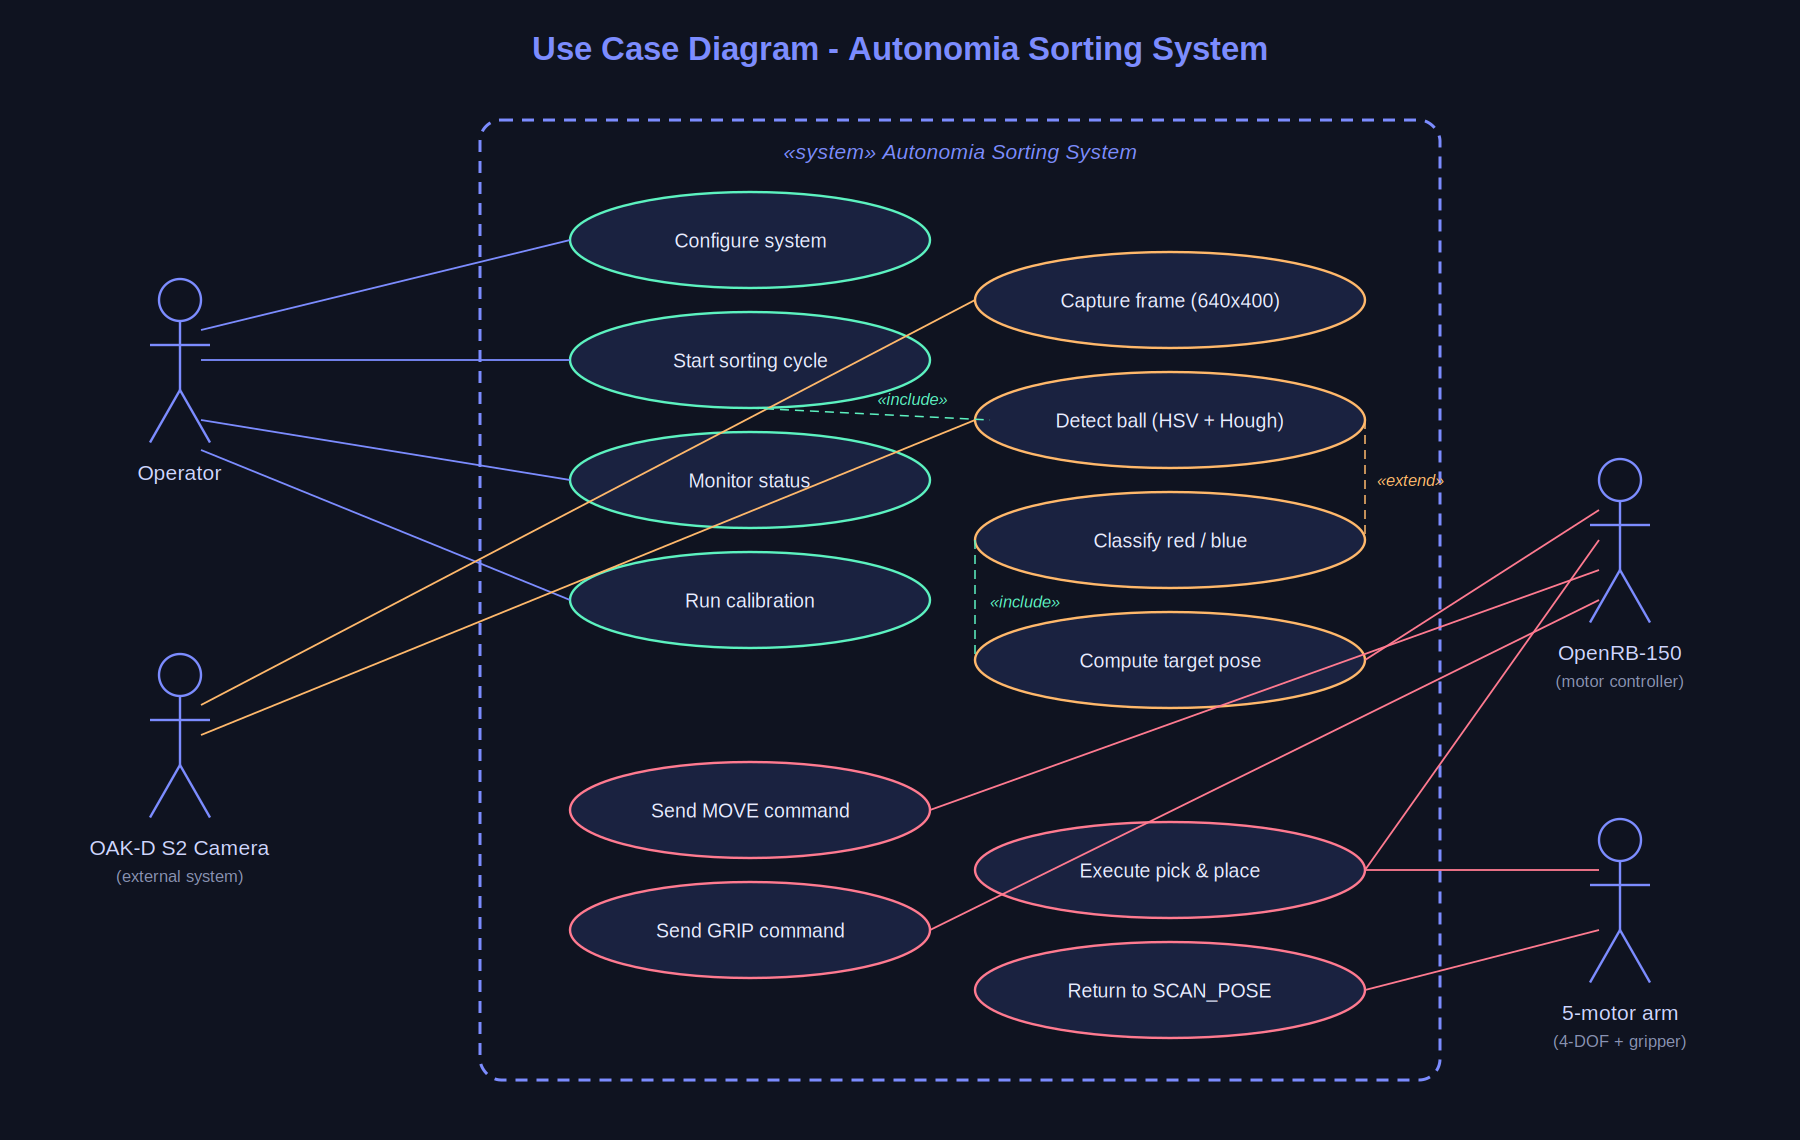
\includegraphics[width=\textwidth]{res/Figures/Diagrams/01_use_case.png}
    \caption{Use case diagram of the Autonomia sorting system.}
    \label{fig:use-case-diagram}
\end{figure}

\clearpage

\subsection{Diagram 2 -- Activity Diagram}
\label{app:activity-diagram}

The activity diagram shows one full pick-and-place cycle as a sequence of activities. The cycle is the unit
of work the system performs over and over: detect a ball, classify it, pick it up, place it in the right bin,
log the result, and start again.
The cycle starts with Initialise system at the top. The next step is Capture frame, where the camera
delivers one image to the Pi. The frame is preprocessed (CLAHE plus HSV conversion) and then run
through the detection pipeline (HSV masks plus the Hough Circle Transform). A diamond decision (Ball
detected?) is the only branch in the diagram. If no ball is detected, the activity loops back to Capture
frame on the dashed line; the system waits for a new frame and tries again. If a ball is detected, the
activity continues downward.
Below the diamond, the system classifies the ball as red or blue, computes the target pose using
inverse kinematics, moves the arm, picks the ball, and places it in the correct bin. The final activity is
the return to the start pose, after which the cycle ends. In normal operation, ending the cycle
immediately means starting the next one, but the diagram shows a single cycle to keep it readable.
The colours match the system architecture (see Diagram B.5). Green outlines mark vision steps
(capture, preprocess, detect, classify). Red outlines mark motion steps (move, pick, place, return). Blue
arrows mark the activity flow itself. The dashed loop is a special case: it is the no branch of the decision,
and a dashed line makes it visible without competing with the main downward flow.
The diagram is updated from the original to include CLAHE in the preprocessing step and to mention
HSV plus Hough as the detection method. The original used a generic Process frame box that did not
say what the processing actually was. The names in the present version match the steps described in
Sections~\ref{sec:image-processing} (image processing) and~\ref{sec:object-detection} (object detection) of the main report, so a reader who wants to
know what CLAHE does can read the matching section without guessing where to look.

\begin{figure}[htbp]
    \centering
    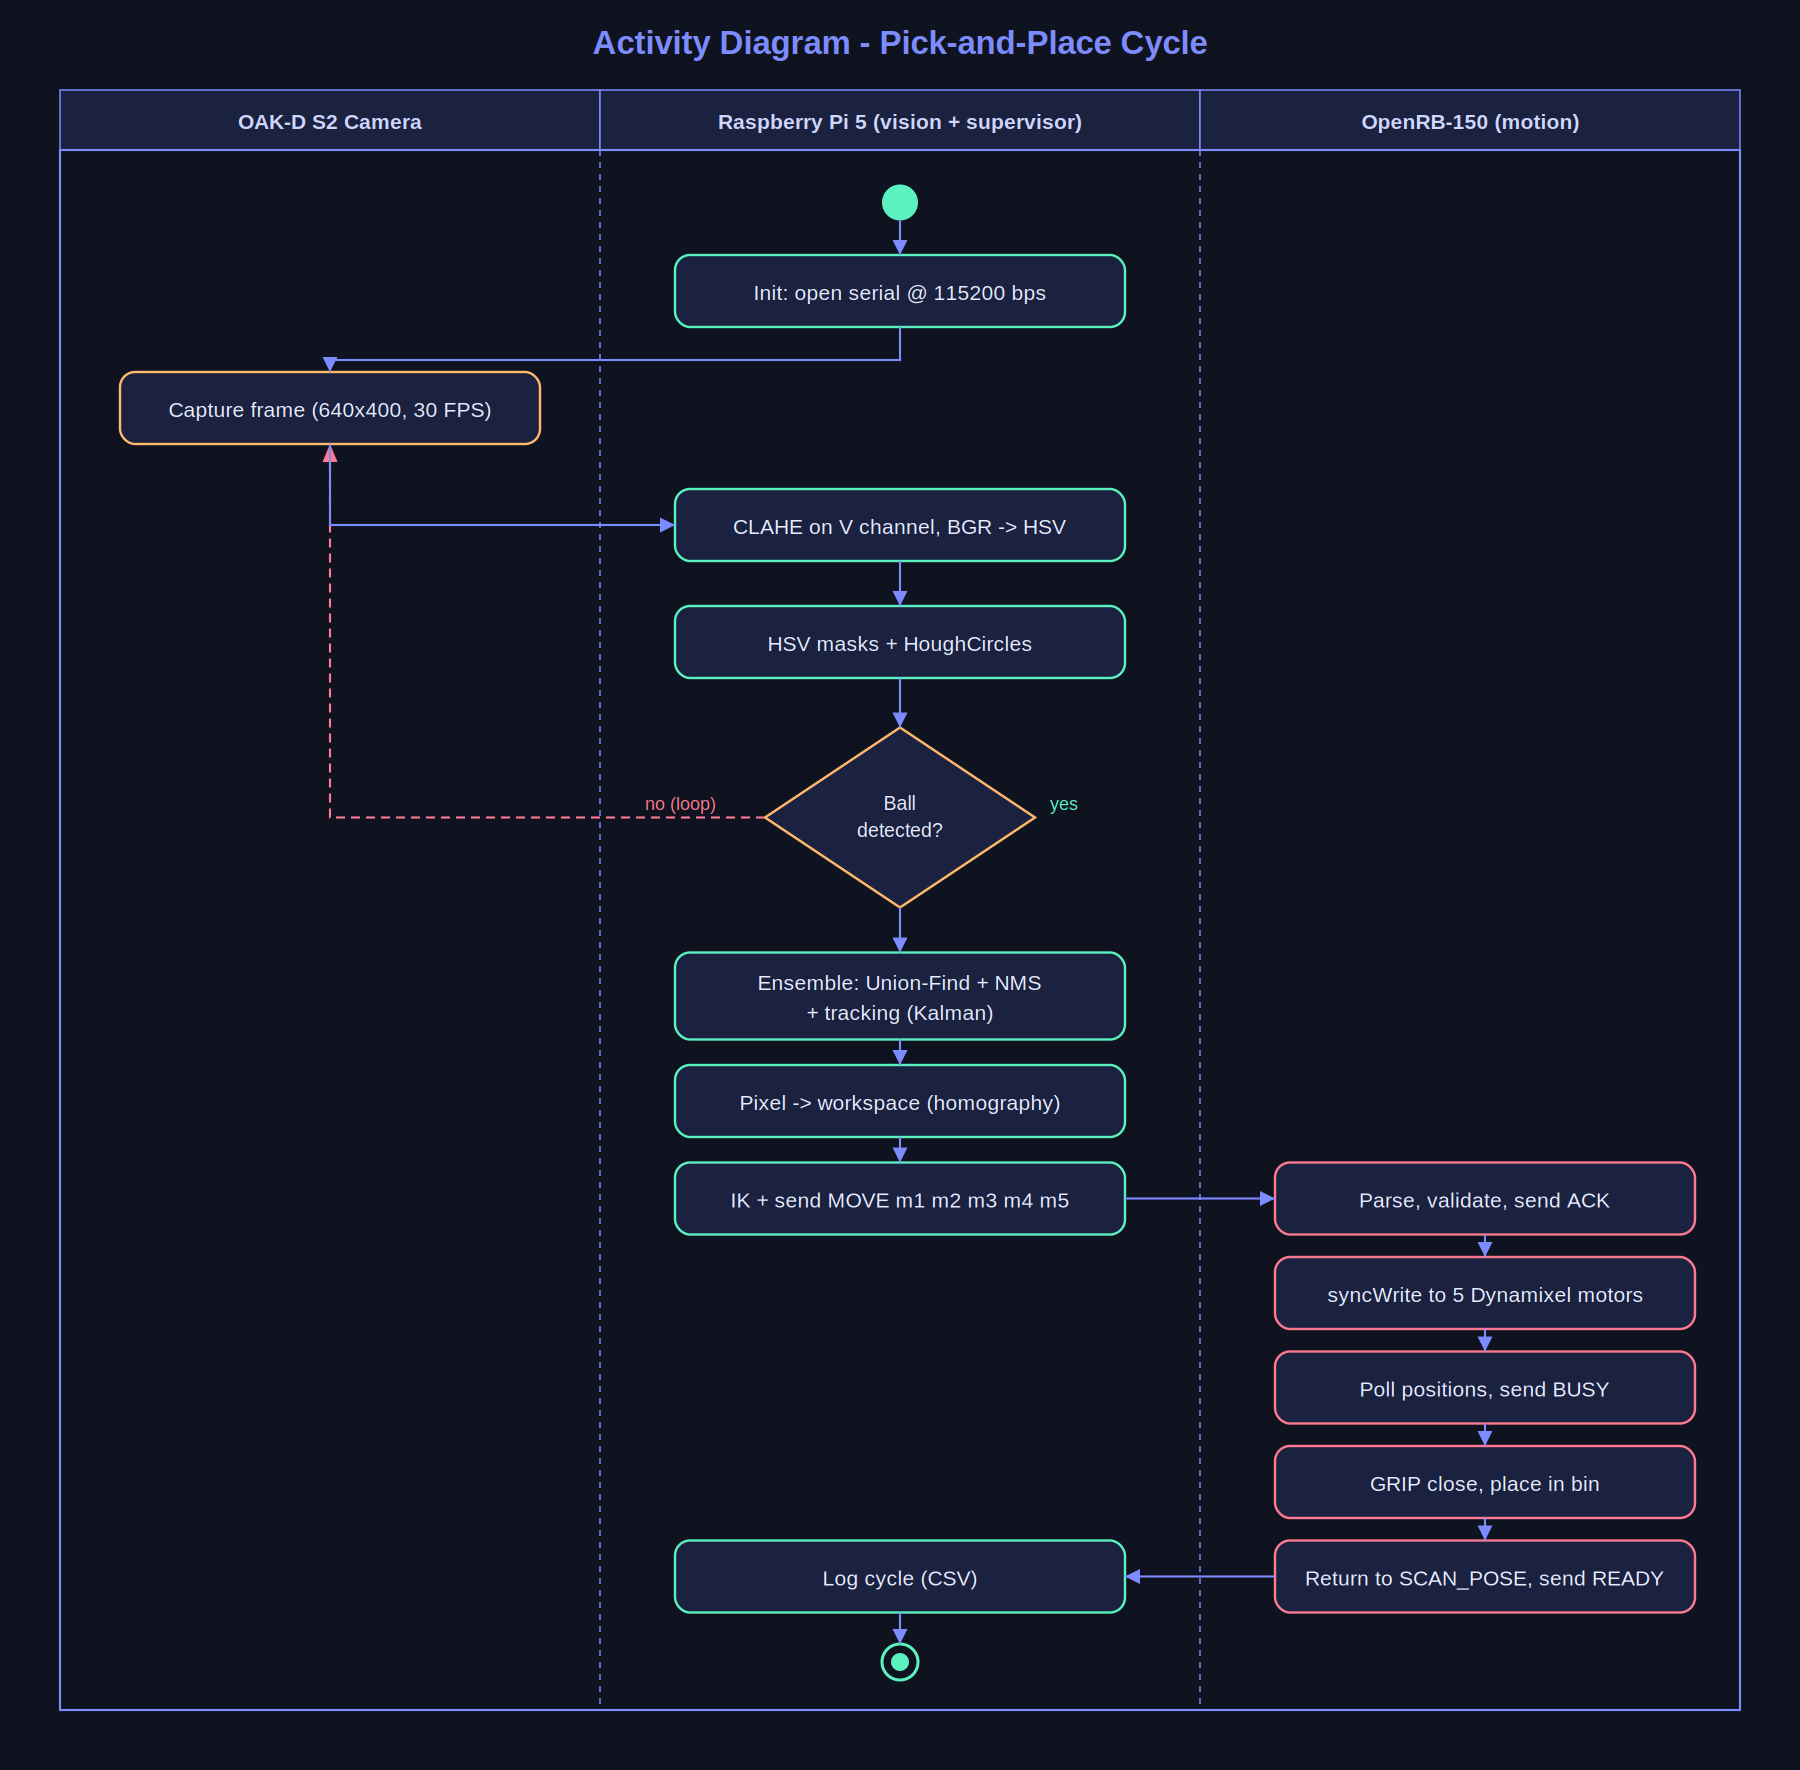
\includegraphics[width=\textwidth]{res/Figures/Diagrams/02_activity.png}
    \caption{Activity diagram of one sorting cycle, with swim lanes for the camera, the Pi, and the OpenRB-150.}
    \label{fig:activity-diagram}
\end{figure}

\clearpage

\subsection{Diagram 3 -- Sequence Diagram}
\label{app:sequence-diagram}
The sequence diagram shows the time-ordered messages exchanged during a single pick-and-place
operation. Time runs from top to bottom. Each vertical dashed line is a lifeline: a participant in the
conversation that exists for the duration of the cycle.
Four lifelines are included: the Operator, the Vision pipeline, the Controller, and the Arm and motors.
Each one corresponds to a different process or device in the system. The activation bars (the thick
rectangles on the lifelines) show when each participant is actively doing work, as opposed to waiting
for a message.
Reading the diagram from the top: the Operator sends start-cycle to the Vision pipeline. The Vision
pipeline calls detect-ball, processes one frame, and returns a detection (colour and position) to the
Operator. The Operator passes the detection to the Controller via pick-ball, which then commands the
Arm and motors to move to the target. When the arm is in position, the Controller sends a closegripper command, places the ball, and returns to the start pose. The Arm reports back when the
operation is complete. A final log entry is written and the cycle ends.
The diagram uses four high-level lifelines to keep the figure readable. The firmware-level message flow
(ACK, BUSY, READY, MOVE m1 m2 m3 m4 m5) is described in Section~\ref{sec:comm} of the main report, where it
has the space to be shown properly. A reader who needs the wire-format details goes to that section.
A reader who wants the overall flow stops here.
Solid arrows are synchronous calls; dashed arrows with open arrowheads are return values. The selfcall on the Vision pipeline (the curved arrow that loops back to itself) means "process frame internally"
without exchanging any message. That covers everything between reading the frame and producing
the detection.


\begin{figure}[htbp]
    \centering
    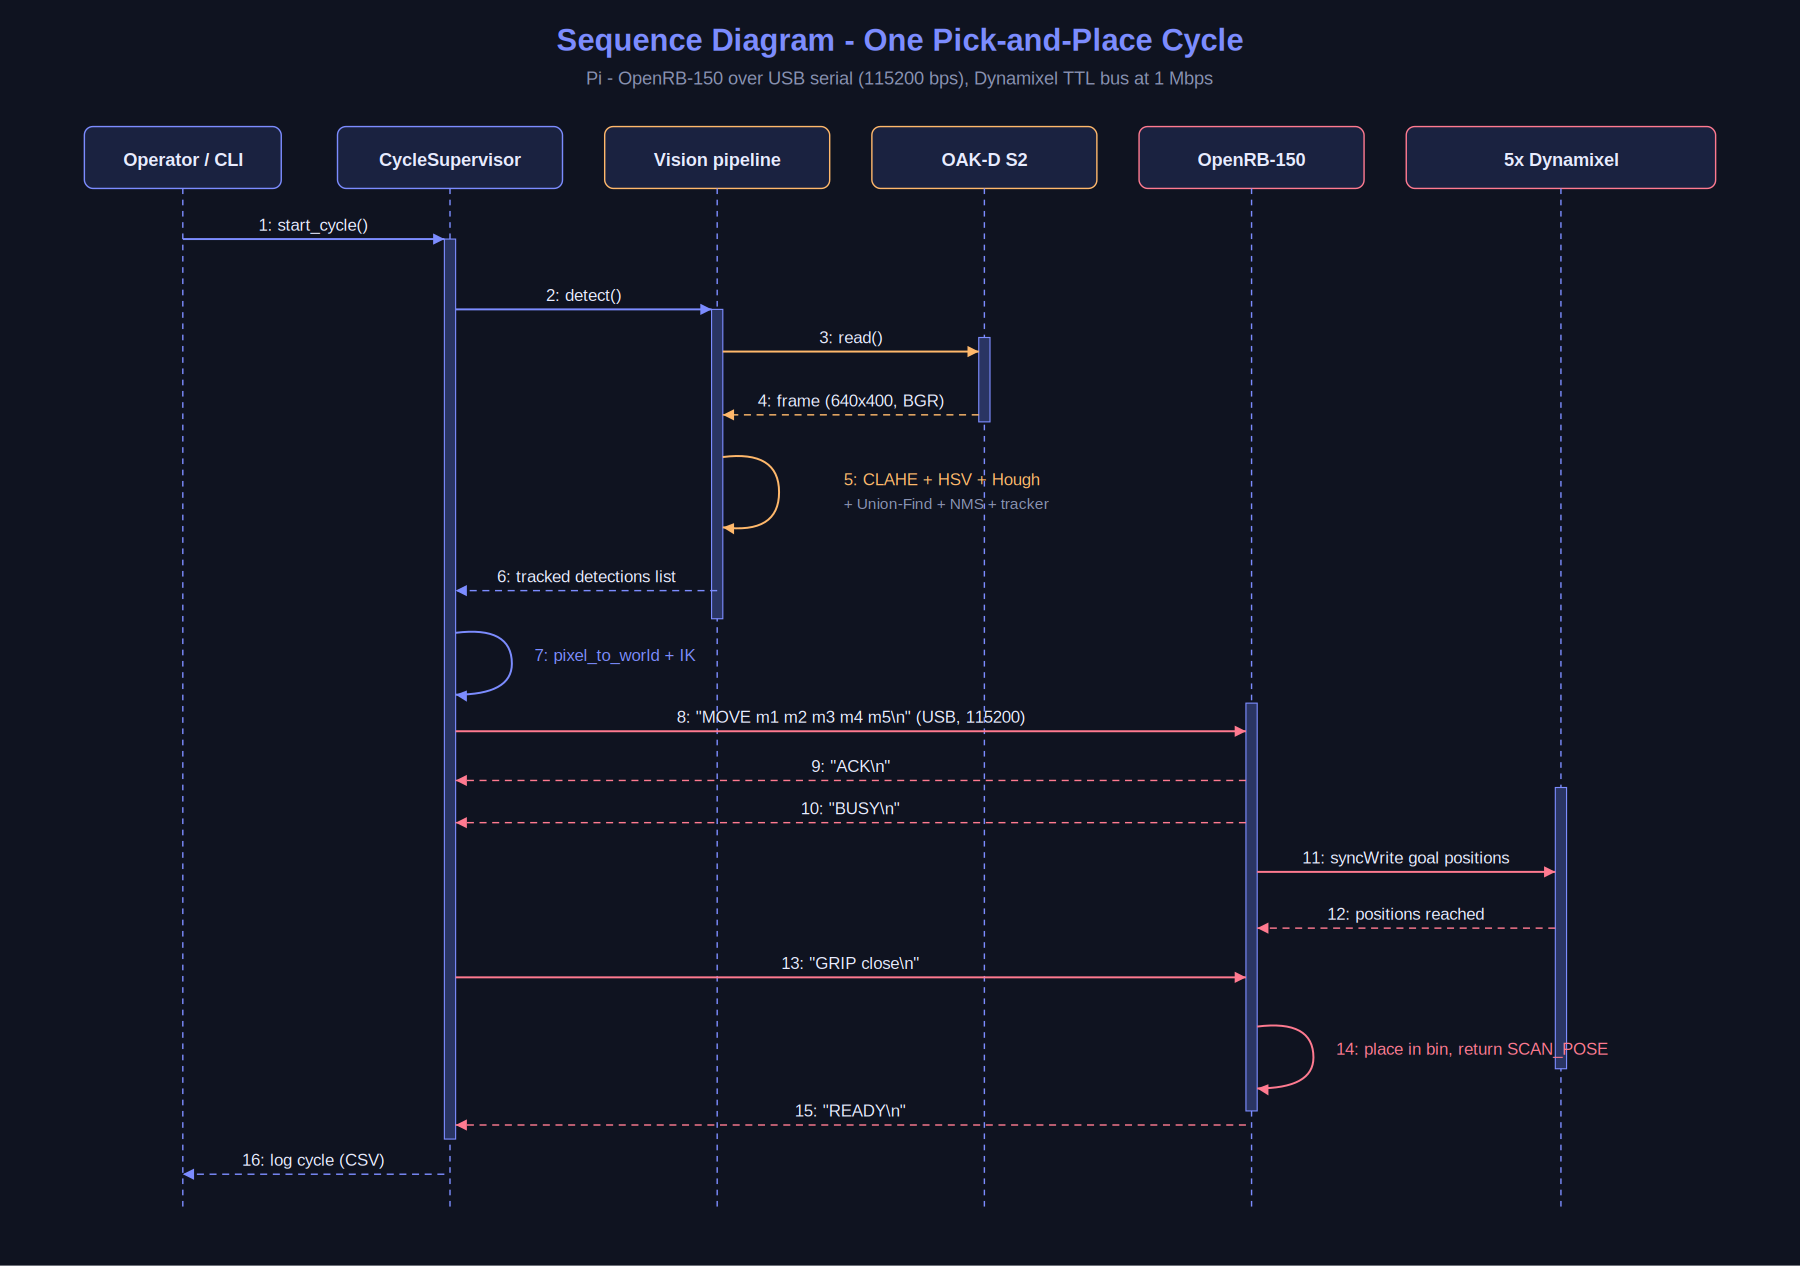
\includegraphics[width=\textwidth]{res/Figures/Diagrams/03_sequence.png}
    \caption{Sequence diagram for one sorting operation.}
    \label{fig:sequence-diagram}
\end{figure}

\clearpage

\subsection{Diagram 4 -- System Architecture}
\label{app:system-architecture-diagram}

The architecture is organised into four layers along the principle of separation of concerns. Each layer
talks only to its adjacent layers via defined interfaces. This split makes each layer testable on its own
and lets us change one layer without rewriting the others.
The Application layer holds the cycle supervisor, the operator CLI, and the logger. These are the toplevel Python modules that an operator interacts with. The supervisor is the state machine that drives
the whole cycle; the CLI is the front-end the operator uses to start, stop, or inspect the system; the
logger writes one row per cycle to a CSV file for later analysis.
The Perception layer holds the camera interface, the CLAHE preprocessor, the HSV plus Hough
detector, and the tracker. The layer takes raw frames in and produces a list of tracked ball positions
out. Each component does one thing and has a well-defined input and output, which makes the layer
easy to test against pre-recorded video files without the live camera.
The Control layer holds the inverse kinematics solver, the serial protocol, and the firmware on the
motor controller. The IK solver converts target positions in workspace coordinates into goal positions
for the motors. The serial protocol carries the goal positions and the status replies between the Pi and
the controller. The firmware reads the protocol, drives the motors, and reports back. This layer is
where the system goes from abstract coordinates to physical motion.
The Hardware layer holds the physical camera, the motors and gripper, and the power supply. The
diagram shows these as generic boxes; the specific models are listed in the hardware section of the
main report. Keeping the names generic in the diagram means the diagram does not need to be
updated when a motor is replaced, only the table.
The diagram replaces an earlier version that listed components no longer in the system (SQLite
database, REST API, Tkinter dashboard) and used the wrong motor controller. The present version
reflects what is actually built. The arrows between the layers are solid because the data flow is direct:
each layer hands its output to the layer below, and nothing skips layers.

\begin{figure}[htbp]
    \centering
    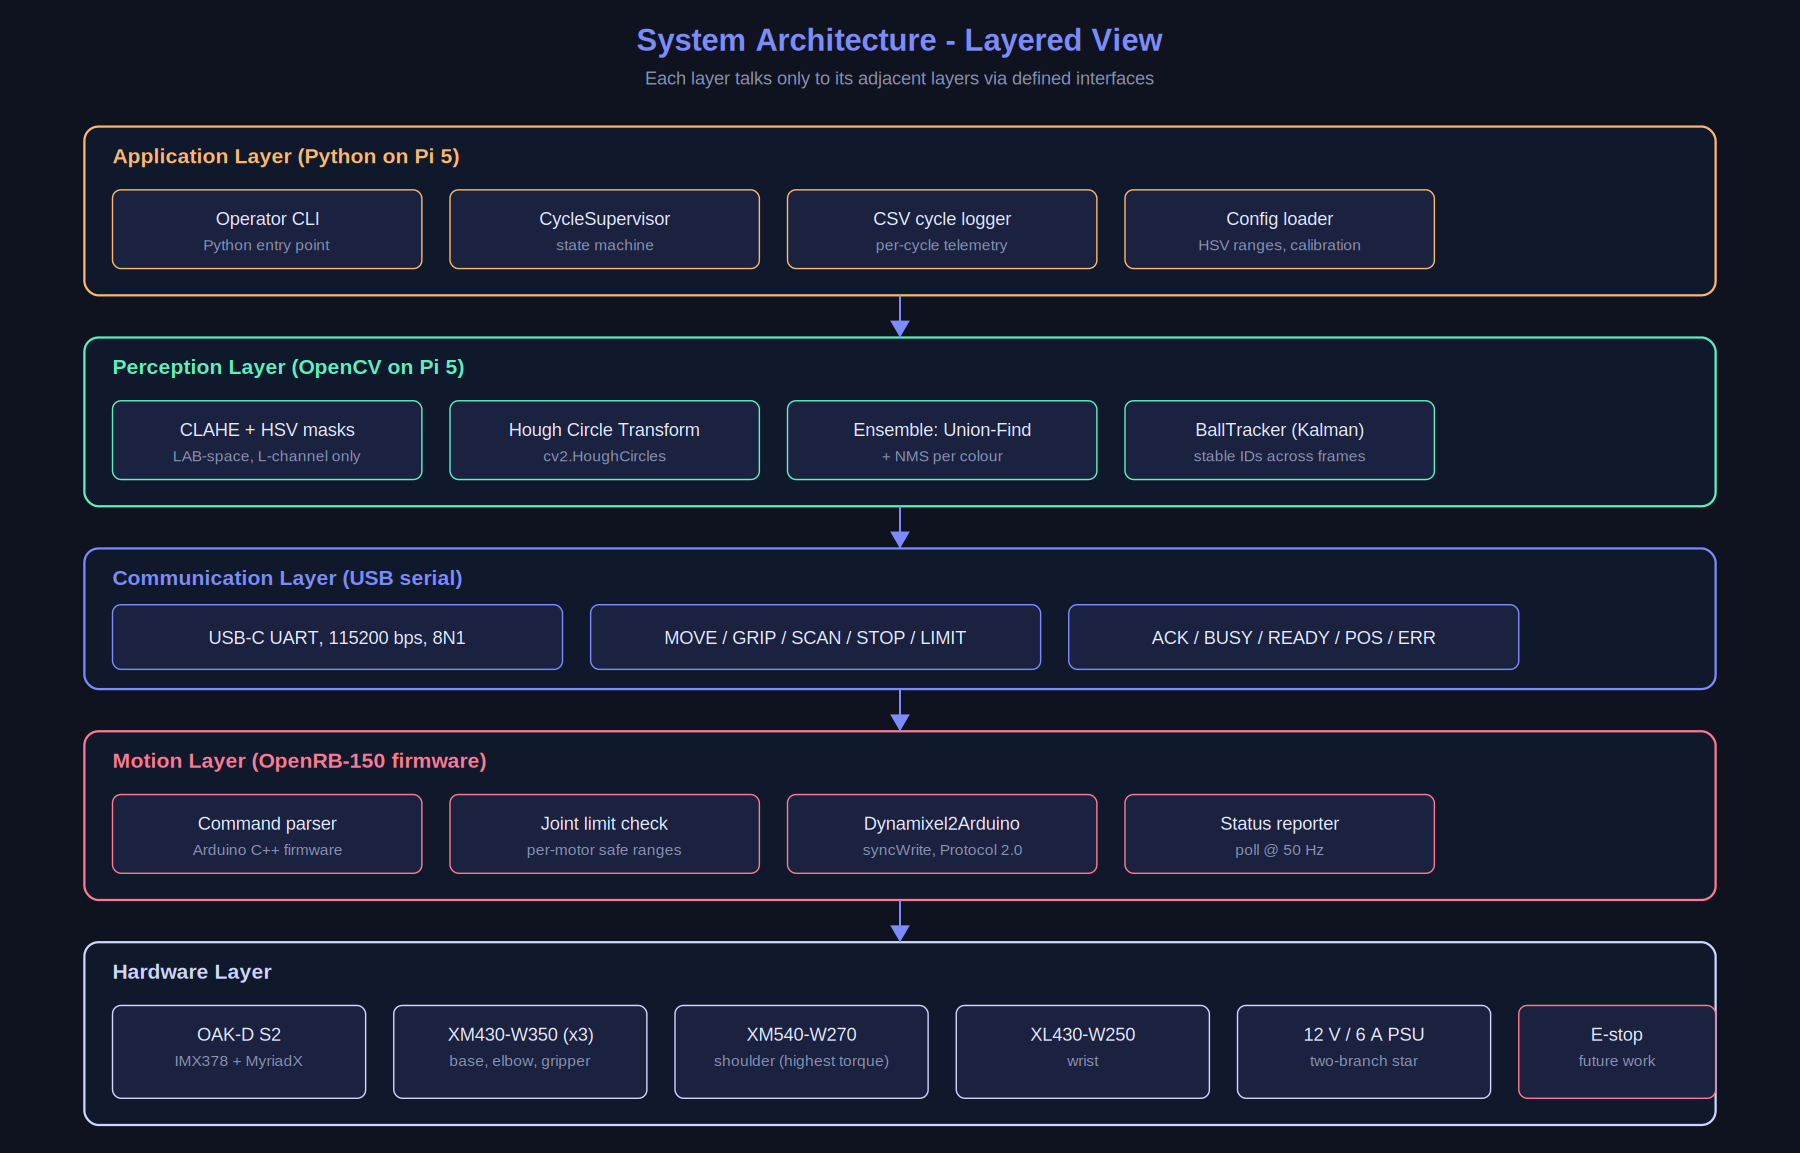
\includegraphics[width=\textwidth]{res/Figures/Diagrams/04_system_architecture.png}
    \caption{Layered system architecture.}
    \label{fig:system-architecture-diagram}
\end{figure}

\clearpage

\subsection{Diagram 5 -- Black Box Diagram}
\label{app:black-box-diagram}

The black box view shows the system as a single unit with its external inputs and outputs. It is included
so the report can be read top down before any internal structure is introduced. A reader looking at this
diagram should be able to describe the purpose of the system in one sentence, without knowing how it
works on the inside.
There are four inputs. The video stream comes from the camera over USB 3.0. The operator command
starts and stops the cycle through the Python CLI. The power supply provides 12 V to the motors and 5
V to the Raspberry Pi. The balls themselves are the physical objects to be sorted; they enter the system
by being placed on the workspace mat.
There are four outputs. A sorted ball ends up in the correct bin: this is the primary outcome of the
system, the reason the project exists. A status text appears on the operator terminal so the operator
knows what the cycle is doing in real time. A cycle log is written to disk as a CSV file with one row per
cycle: this is the evidence used for the testing chapter. The arm motion itself is an output in the
physical sense: the arm moves while the cycle is running, even though motion is not a deliverable that
anyone can hold or read.
The black box view does not show how the work is done. Section~\ref{sec:system-architecture-overview} of the main report describes the
high-level architecture that opens the box. Section~\ref{sec:software-architecture} describes the software architecture, Section~\ref{sec:hardware-architecture}
the hardware, and Section~\ref{sec:data-flow} the data flow. The layered view in Figure~\ref{fig:system-architecture-diagram} is the next step down from
this diagram, and the implementation chapter goes the rest of the way to the source code.

\begin{figure}[htbp]
    \centering
    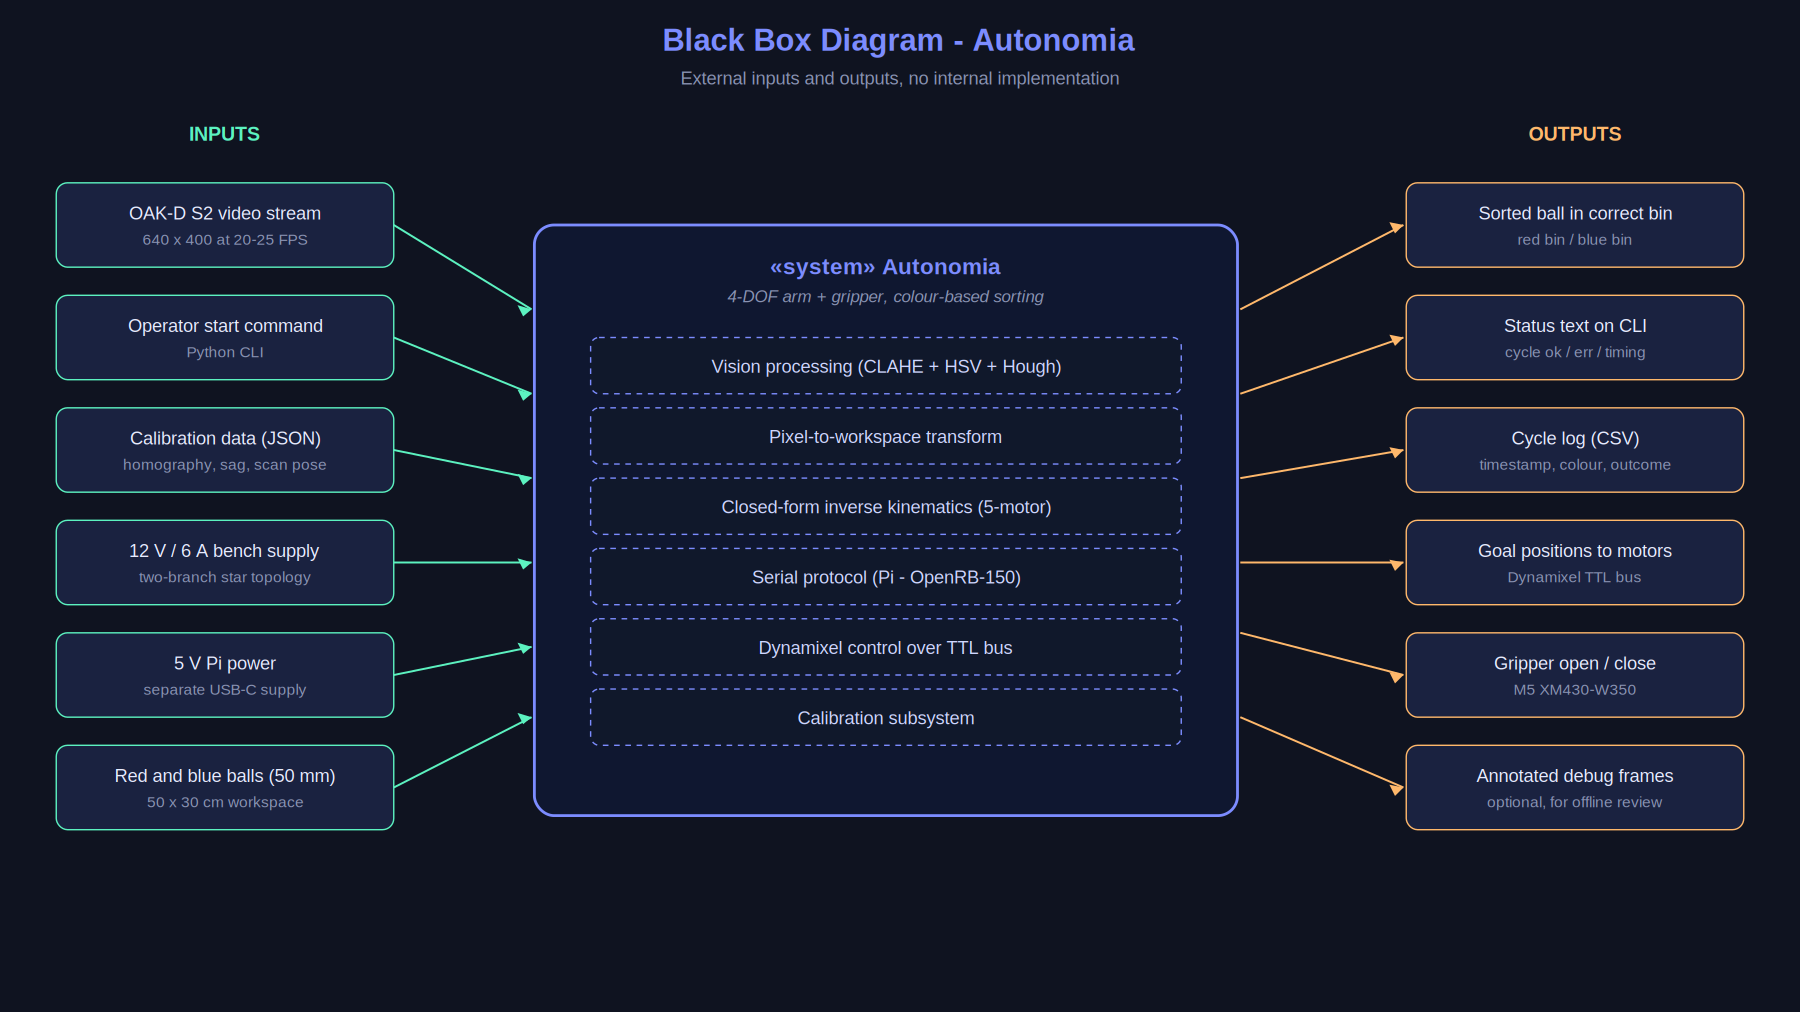
\includegraphics[width=\textwidth]{res/Figures/Diagrams/05_black_box.png}
    \caption{Black box view of the Autonomia system.}
    \label{fig:black-box-diagram}
\end{figure}

\clearpage

\subsection{Diagram 6 -- Stakeholder Diagram}
\label{app:stakeholder-diagram}

The stakeholder diagram groups all parties involved in or affected by the project into three rings:
primary, secondary, and tertiary. The grouping informs the priority of requirements: a need from a
primary stakeholder takes precedence over a need from a tertiary stakeholder when the two conflict.
The grouping also informs the audience for documentation: the supervisor reads the report, the future
employer reads the abstract, and the open source community sees the published code.
The primary stakeholders are the Project group, the Supervisors, and the External supervisor. These
three are directly involved in the day-to-day work of the project. They evaluate the deliverables, point
out problems, and have the strongest say in what is built. The diagram places them in the innermost
ring because they are the ones whose needs the system has to satisfy first.
The secondary stakeholders are the Examiner, USN, future employers, and fellow students. They
evaluate the result or are served by it without contributing directly to the work. The examiner reads
the report and watches the demonstration during the bachelor defence. USN as an institution owns
the equipment, the workspace, and the academic record. Future employers may read the report or see
the demonstrator as part of a job interview. Fellow students see the work during the bachelor defence
and may use parts of it in their own projects later.
The tertiary stakeholders are the component suppliers, IT services, the open source community, and
the wider automation industry. They have an indirect or contextual interest. Suppliers benefit from the
project as a customer reference. IT services provide the network and laboratory infrastructure without
being involved in the technical work. The open source community provides the libraries the project
depends on (OpenCV, DepthAI, Dynamixel2Arduino, numpy, scipy). The wider automation industry is
the long-term context that the project sits in, although no specific company is part of the work.
The numbers in the diagram match the rows of the stakeholder table in Section~\ref{sec:team} of the main report.
The roles are kept generic so the diagram does not need to be updated when individual people change.
The names are listed in the table and in the acknowledgements at the front of the report.


\begin{figure}[htbp]
    \centering
    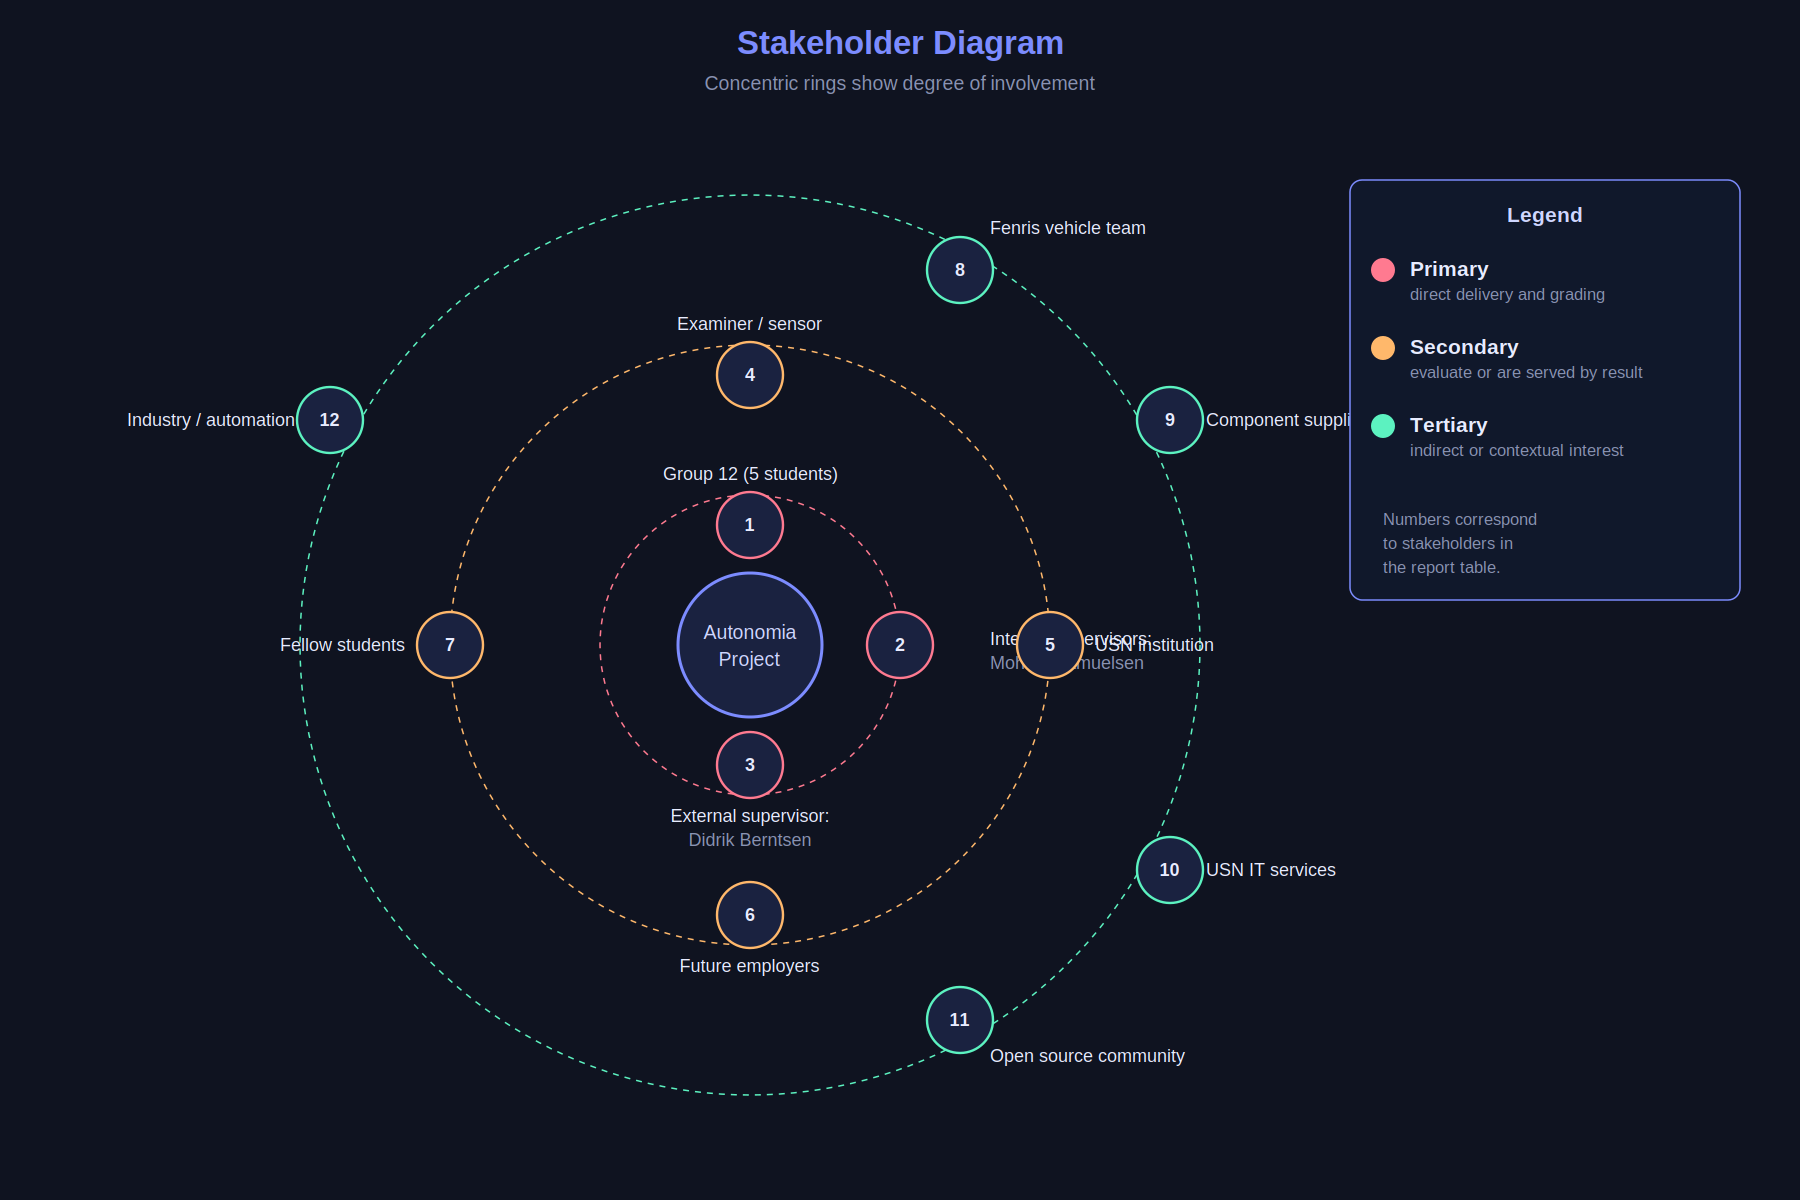
\includegraphics[width=\textwidth]{res/Figures/Diagrams/06_stakeholders.png}
    \caption{Stakeholder diagram. Concentric rings show degree of involvement.}
    \label{fig:stakeholder-diagram}
\end{figure}

\clearpage

\subsection{Diagram 7 -- Key Performance Parameters}
\label{app:kpp-diagram}
The KPP diagram presents the six measurable success criteria the system is evaluated against. Each
row shows the parameter, the target, and the measured value where one exists. The bars are not to
exact scale; they show roughly where the result sits relative to the target. The figure is meant for a
quick scan, not for precise reading.
KPP-01 is the ball detection rate. The target is 90 percent or better. The measured value is 98 to 100
percent under controlled lighting at 300 to 700 lux. The number comes from the testing chapter,
where the pipeline is exercised against a fixed test set with hand-labelled ground truth.
KPP-02 is the vision pipeline throughput. The target is 15 FPS or better, which is the lower bound for
real-time operation in the project context. The measured value is 20 to 25 FPS on the Raspberry Pi 5 at
640 by 400 resolution. The measurement was made with per-stage profiling so we know which stage of
the pipeline dominates the runtime; CLAHE and HoughCircles together account for about 70 percent of
the per-frame time.
KPP-03 is the false positive rate. The target is less than 5 percent. The measured value is below 2
percent across the test set. The ensemble step (Union-Find plus Non-Maximum Suppression,
described in Section~\ref{sec:ensemble}) is the main reason the rate is this low: it filters out detections that one
method picked up but the other did not.
KPP-04 is position accuracy at the workspace. The target is 1 cm or better at all tested reach distances.
This is a goal value from the inverse kinematics calibration; the actual error depends on the reach
distance and on how recently the touch calibration was run. Sections~\ref{sec:ik-solver} and~\ref{sec:calibration} of the main report
describe the solver and the calibration procedure that together support this number.
KPP-05 is the steady-state cycle time. The target is 8 seconds or less per cycle. The bar in the diagram
shows roughly where the system sits at the time of writing, on the order of 6 to 7 seconds depending
on the trajectory. The remaining gap to the goal value is being measured in the final week of testing.
KPP-06 is continuous uptime without operator action. The target is 30 minutes or more. The number is
intended to demonstrate that the system can run a full bin worth of balls without intervention. The bar
shows the current state; full-duration runs are part of the validation phase described in Section~\ref{sec:development-phases}.
Three of the six KPPs (KPP-01, KPP-02, KPP-03) have measured values above the target at the time of
writing. The other three are works in progress. The testing chapter (Chapter~\ref{cha:testing}) is the source of truth
for the final numbers; this diagram is the quick reference that points back to it.


\begin{figure}[htbp]
    \centering
    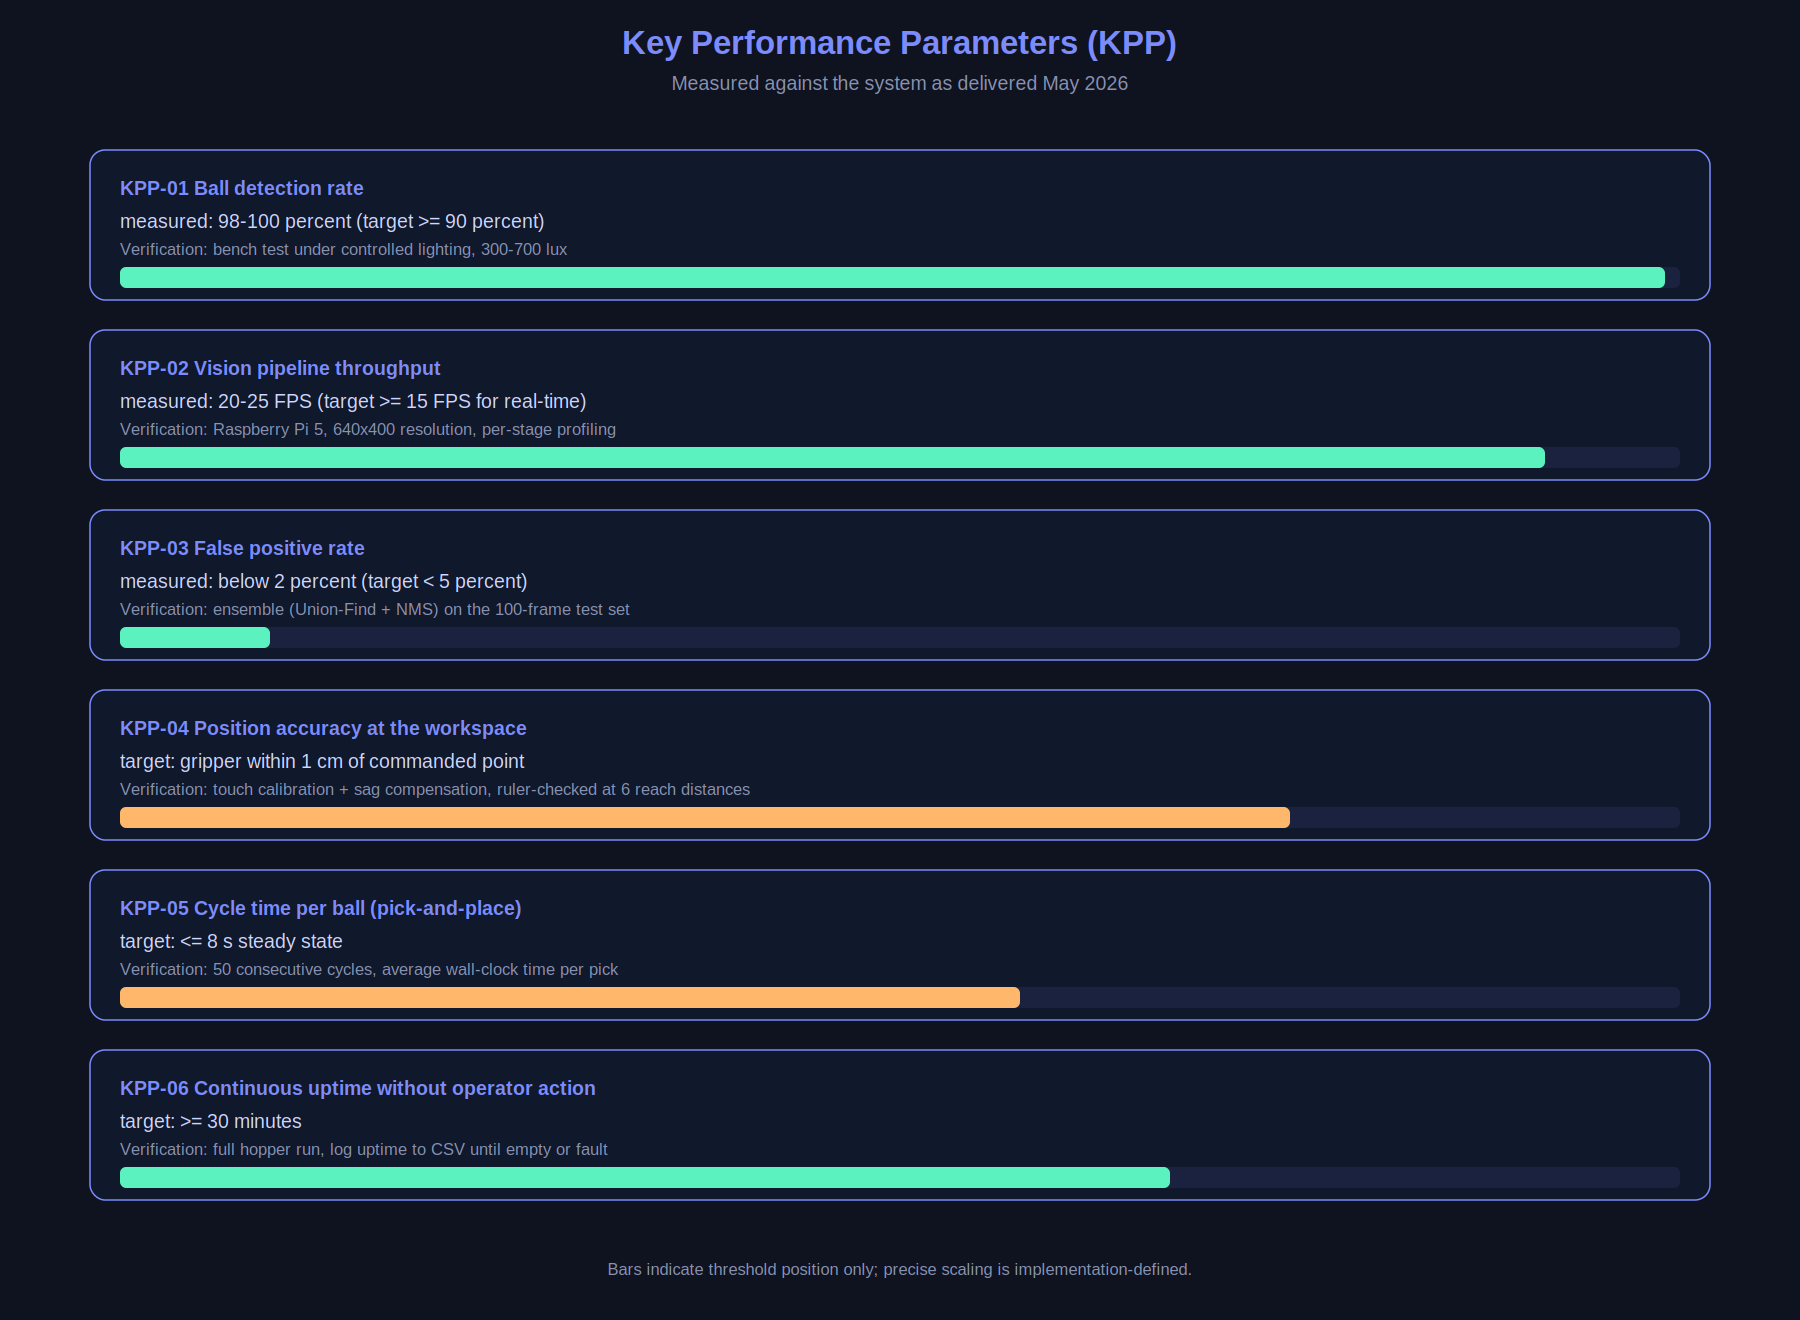
\includegraphics[width=\textwidth]{res/Figures/Diagrams/07_kpp.png}
    \caption{Key performance parameters with thresholds and measured values.}
    \label{fig:kpp-diagram}
\end{figure}

\clearpage

\subsection{Diagram 8 -- Component Diagram}
\label{app:component-diagram}
The component diagram makes the physical distribution of software components explicit. Two nodes
are shown: the Host computer (Python) and the Motor controller (firmware). The single interface
between the nodes is the USB serial link, drawn as a dashed line with sockets at both ends. Solid lines
inside each node are the internal data and control flows.
On the host side, the components map one-to-one to the Python modules described in Section~\ref{sec:software-architecture} of
the main report. The Camera interface wraps the DepthAI API. The Ball detector runs the vision
pipeline (CLAHE, HSV masks, HoughCircles, ensemble merging). The Cycle supervisor is the top-level
state machine. The Inverse kinematics module converts workspace coordinates into motor goal
positions. The Serial bridge owns the USB serial link. The Logger writes the cycle log. The Config and
calibration component sits below the runtime components and is the source of the parameters they all
load at startup.
On the controller side, the firmware is split into five components. The Command parser reads bytes
from USB serial, assembles them into lines, and parses each line into a command and zero or more
integer arguments. The State machine has three states (INIT, READY, FAULT) and decides how to react
to each parsed command. The Joint limit check rejects commands that would drive a motor outside its
safe range. The Motor driver wraps the Dynamixel2Arduino library and sends actual TTL packets to the
motors. The Status reporter sends ACK, BUSY, READY, and ERR replies back over the USB link.
The diagram shows the boundary between the two nodes as a clean line because that is what it is.
Every piece of state, every variable, and every function call lives on exactly one side. The protocol on
the dashed line is the only thing both sides have to agree on. Section~\ref{sec:comm} of the main report describes
the protocol in detail. The two halves can be developed and tested independently, which is the main practical reason for the split: the firmware is exercised by a small Python script that simulates a Pi, and
the Pi-side code is exercised against pre-recorded protocol traces without the firmware running.
Component names are generic on this diagram (Camera interface, Ball detector, Inverse kinematics)
rather than the specific class names from the source code (OAKCamera, SimpleBallDetector, ArmIK).
The class names appear on Diagram B.10 (the class diagram), which is the right level for them. A reader
who follows both diagrams can go from a component box on this diagram to a class box on the next
one in a single jump.


\begin{figure}[htbp]
    \centering
    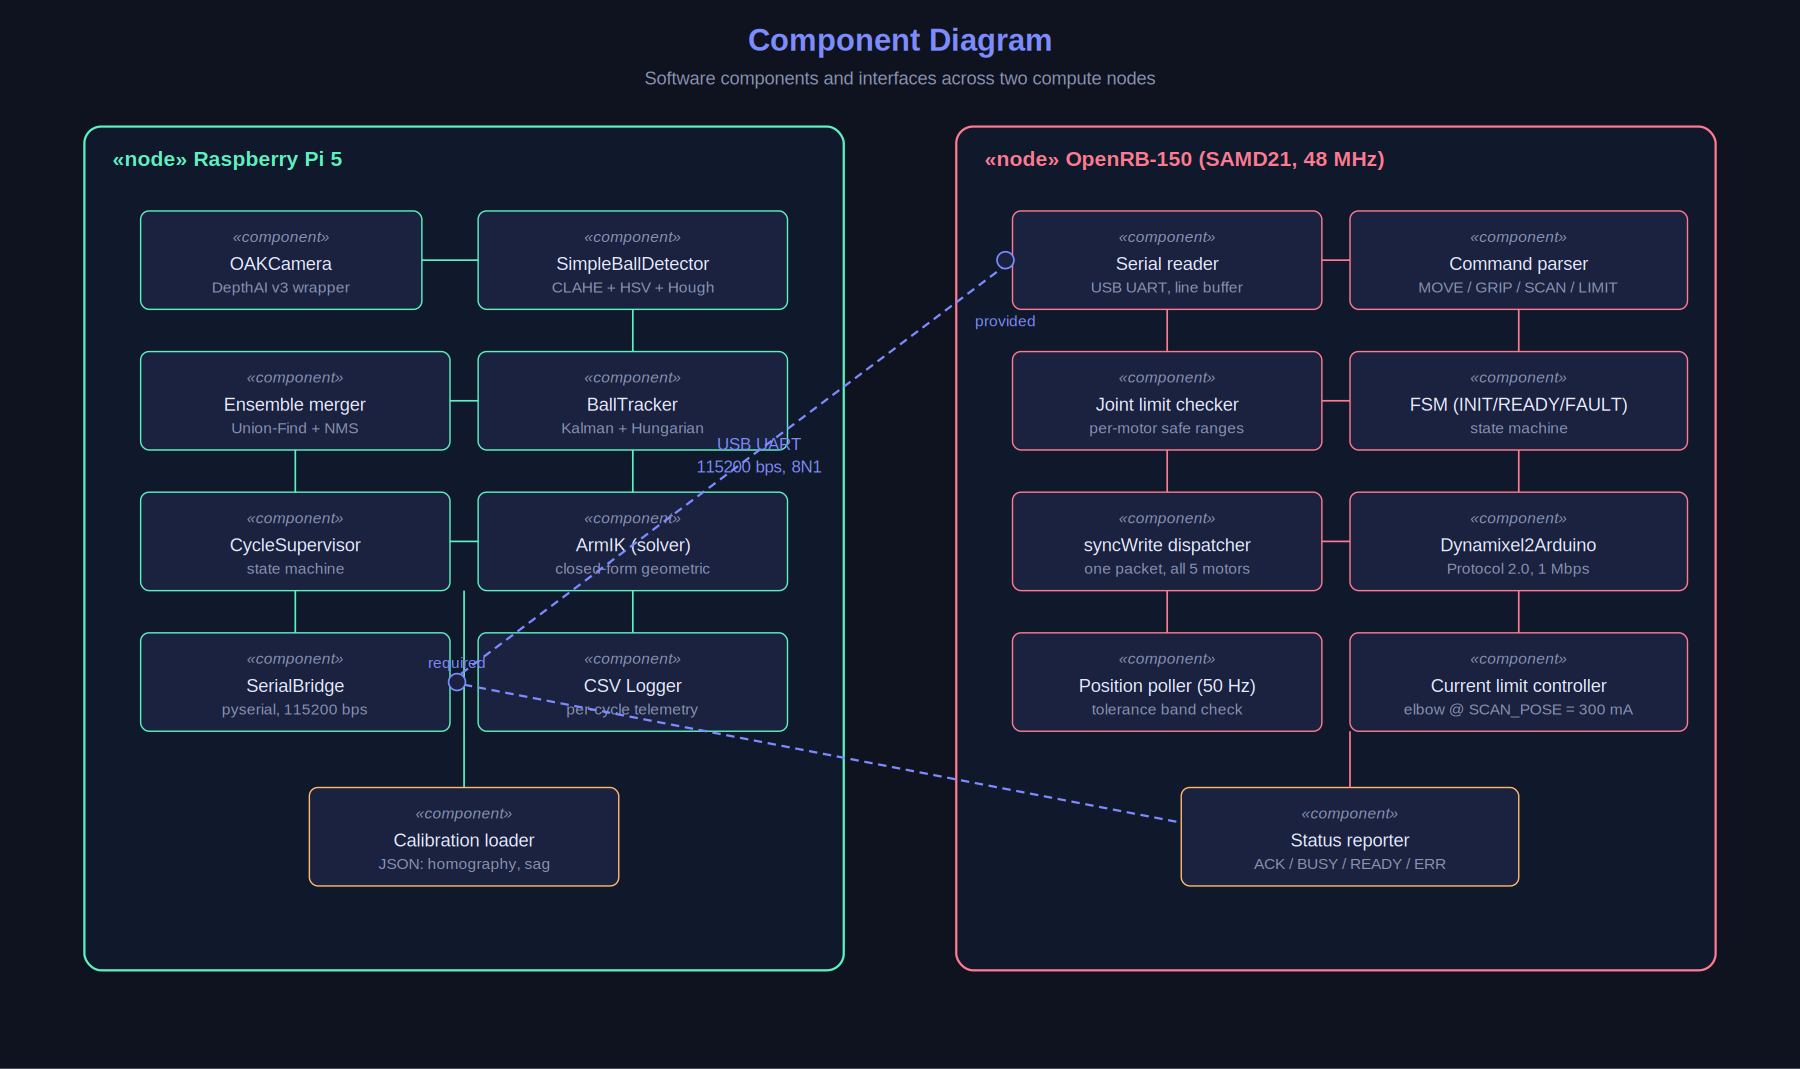
\includegraphics[width=\textwidth]{res/Figures/Diagrams/08_component.png}
    \caption{Component diagram across the Pi and OpenRB-150 nodes.}
    \label{fig:component-diagram}
\end{figure}

\clearpage

\subsection{Diagram 9 -- Class Diagram}
\label{app:class-diagram}
The class diagram covers the host-side software. The firmware is written in C++ using the Arduino
setup and loop pattern, which does not map cleanly to an object-oriented class diagram. The firmware
structure is described in prose in Section~\ref{sec:actuator-control} of the main report instead.
Seven classes are shown. CycleSupervisor sits at the top and owns four collaborators: the Camera, the
BallDetector, the BallTracker, and the SerialBridge. The class names match the import statements in
the source code, so an examiner can go from a class in the diagram to the matching file in the
repository without searching. Attributes start with a minus sign (private), methods with a plus sign
(public), following standard UML notation. The notation is the same as is taught in any first-year
software engineering course.
The CycleSupervisor is the entry point. Its run() method is what gets called when the operator starts
the system. The method enters an infinite loop that calls run-once() once per cycle. run-once() asks
the BallDetector for a list of detections, picks one as the target, runs ArmIK.solve() to get motor
positions, and sends the motion through the SerialBridge. The flow matches the supervisor description
in Section~\ref{sec:software-architecture}.
The BallDetector runs the per-frame pipeline. Its detect() method returns a list of Detection objects:
one per ball seen. The private methods run-hsv(), run-hough(), and ensemble() correspond to the
three stages of the pipeline described in Section~\ref{sec:object-detection} of the main report. Keeping them as private
methods of the same class means the data they share (the colour masks, the contour list) does not
need to be passed around as function arguments.
The Detection class is a dataclass: a simple data container with no behaviour beyond getting and
setting fields. It has the ball's colour, the pixel coordinates of its centre, the radius in pixels, and the
confidence score from the ensemble step. The to-world(H) method converts the pixel position to
workspace coordinates using the homography from the touch calibration; this is the single place in the
host code where the conversion happens.
The SerialBridge handles all communication with the OpenRB-150 controller. The methods (open,
send-move, send-grip, close) match the protocol tokens in Section~\ref{sec:comm}. Each method writes a line to
the serial port and reads the reply. The class owns the pyserial.Serial object as a private attribute,
which means the rest of the code never touches the raw socket and the protocol details cannot leak
into the supervisor logic.
The BallTracker maintains stable identifiers across frames. Its update() method takes a list of
detections from the current frame and matches each one to a track from the previous frame using a
simple Hungarian-style assignment. Predictions for tracks that are not matched in a new frame are
kept alive for up to max-disappeared frames before being dropped. The tracker is not used in every
cycle: it is mainly for displaying the same ball with the same ID across the debug feed.
The ArmIK class is a pure-function class: a fixed set of parameters (the link lengths L1, L2, L3 and the
joint limits) and two methods that have no side effects. solve(x, y, z) takes a target in workspace
coordinates and returns five Dynamixel goal positions. forward(steps) takes the same five positions
back and returns the expected gripper position; it is used for testing that the inverse and forward
solvers are consistent.

\begin{figure}[htbp]
    \centering
    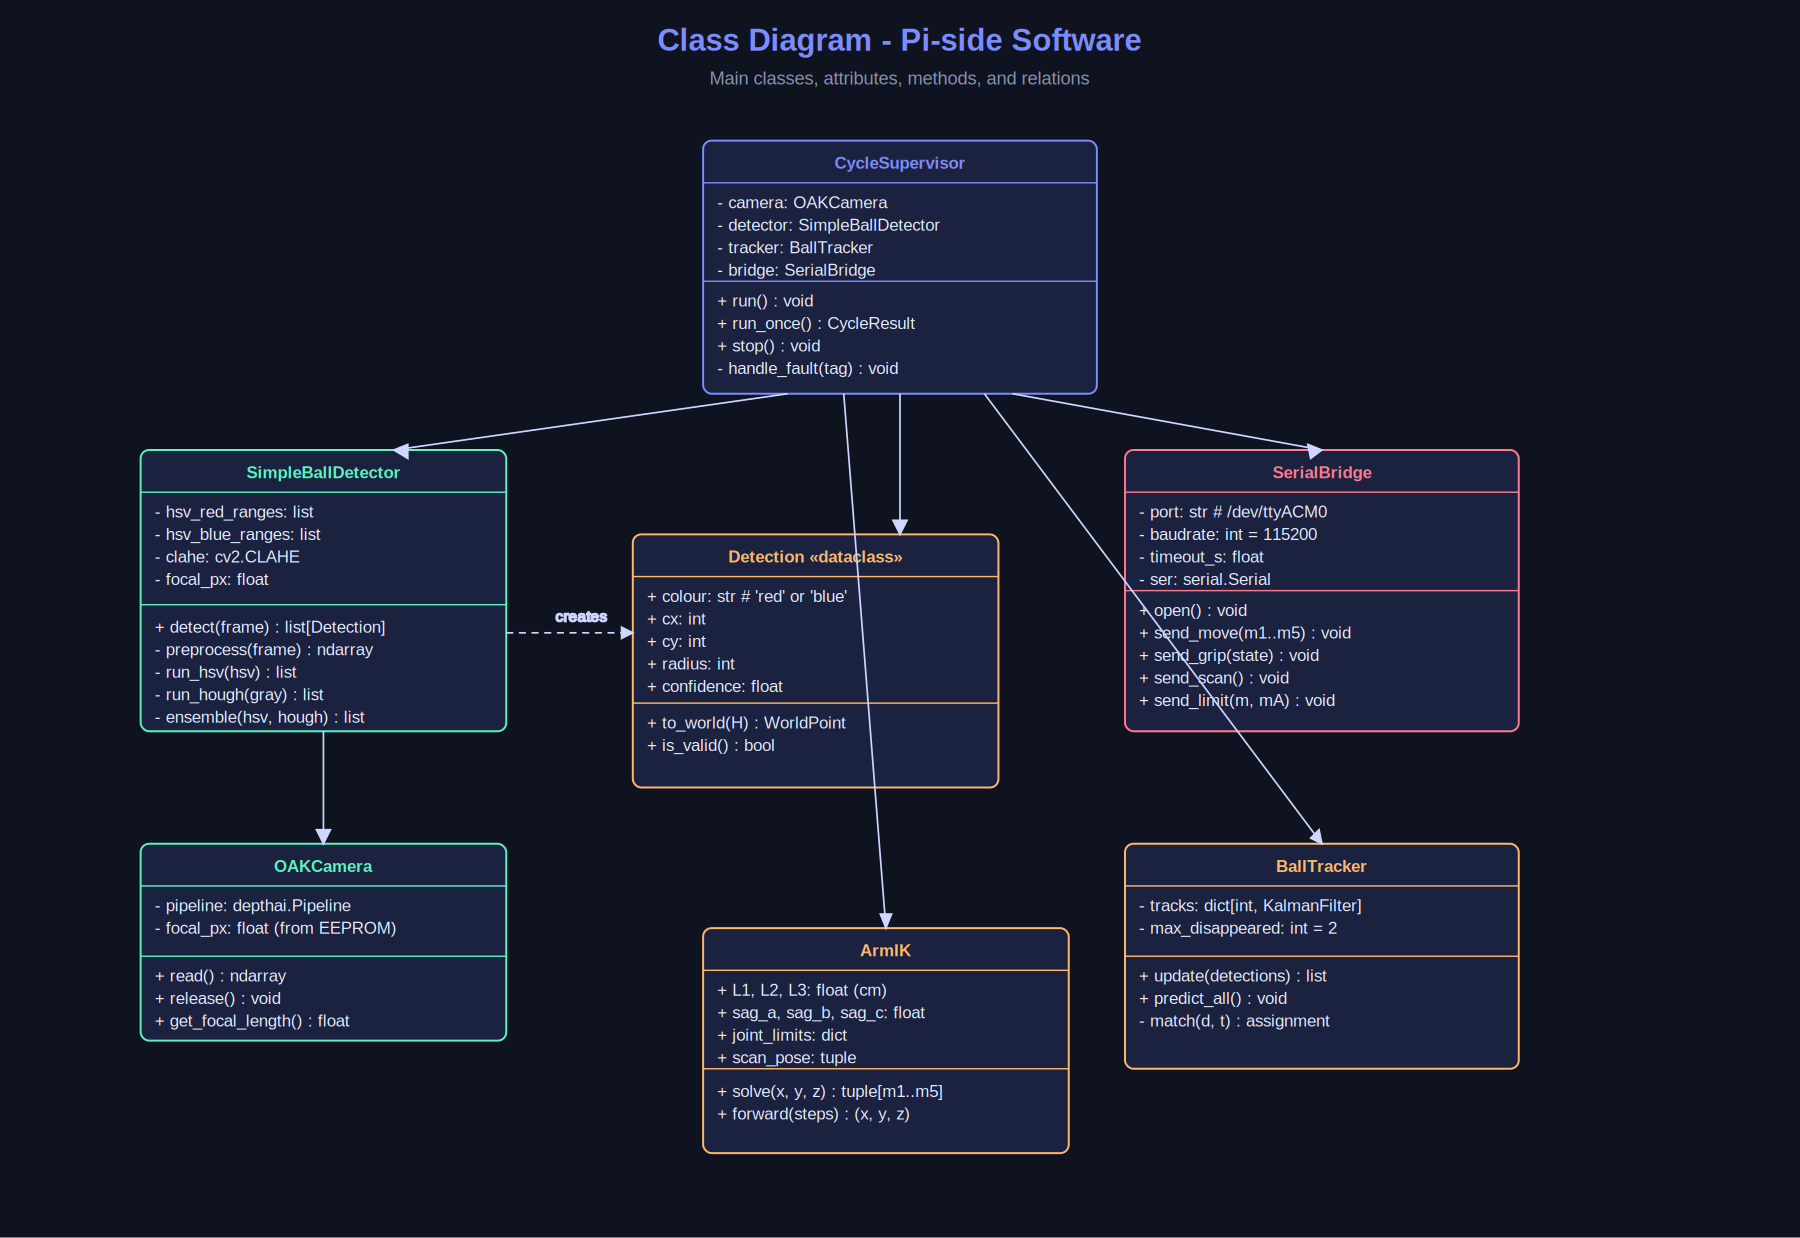
\includegraphics[width=\textwidth]{res/Figures/Diagrams/09_class.png}
    \caption{Class diagram of the Pi-side Python software.}
    \label{fig:class-diagram}
\end{figure}

\clearpage

\subsection{Diagram 10 -- Risk Matrix}
\label{app:risk-matrix-diagram}
This diagram is new and did not exist in the original draft of the diagrams. It visualises every entry in the
risk register from Section~\ref{sec:risk-management} of the main report on the 3 by 3 grid the team uses for risk rating.
The two axes are Likelihood (L) and Consequence (C), each rated on a 1 to 3 scale. The product RI = L x C
gives a risk index between 1 and 9. The matrix has three action classes: low (index 1 to 2), medium (3 to
4), and high (6 to 9). Each cell shows the risk index and the action class. The colours match the action
classes: green for low, yellow for medium, red for high.
All ten risks from Section~\ref{sec:risk-management} are plotted on the matrix. The position of each circle is the (L, C) pair from
the register table. R-01 (schedule slip) is the only risk at the top corner (RI = 9, high). R-02 (IK accuracy),
R-03 (lighting), R-04 (elbow overheating), and R-10 (MobileNetV2, retired) sit at index 6. R-05 (serial
desync) and R-09 (calibration drift) sit at index 4 (medium). R-06 (motor failure) and R-07 (power
supply) sit at index 3 (medium). R-08 (data loss) sits at index 2 (low). R-10 is shown in its retired
position with the (retired) label so the reader can see where it was rated before it was dropped.
The matrix is the single most important figure for the project-management chapter. The examiner can
see at a glance which risks are above the action threshold and which are not. The mapping to action
classes makes the sprint planning rationale visible: high-rated risks are handled this week, mediumrated risks within the next sprint, low-rated risks monitored only. The same logic is described in prose
in Section~\ref{sec:risk-management}, but the diagram shows it in one image.
The matrix also supports the argument in Section~\ref{sec:risk-management} that the project is in a manageable state at the
time of writing. No risks are at the top corner (L = 3, C = 3), and the risks that are at RI = 6 all have
documented mitigations in the register. The risks that started at RI = 9 (notably R-02, which dropped
from 9 to 6 after the inverse kinematics solver and the sag compensation were in place) are no longer
at the top, which is itself evidence of progress.


\begin{figure}[htbp]
    \centering
    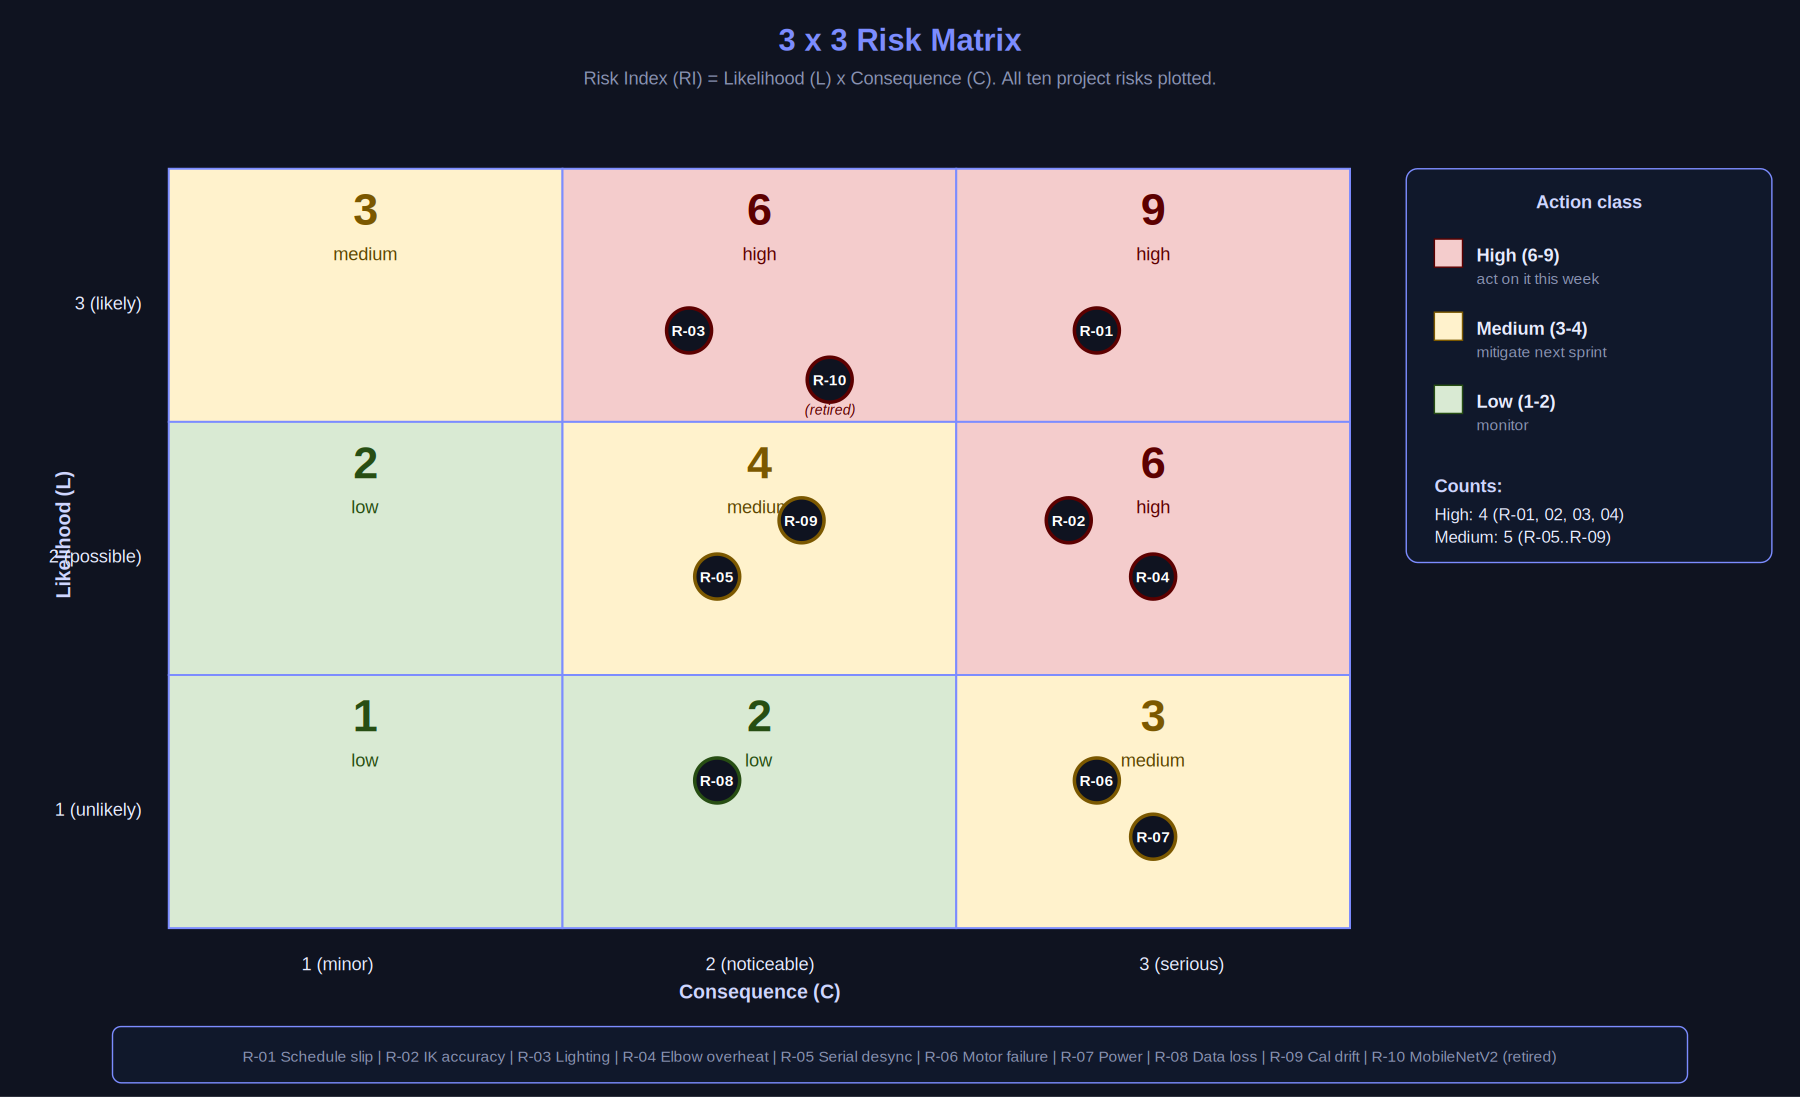
\includegraphics[width=\textwidth]{res/Figures/Diagrams/10_risk_matrix.png}
    \caption{3 by 3 risk matrix with all ten project risks plotted.}
    \label{fig:risk-matrix-diagram}
\end{figure}

\clearpage
